\documentclass[12pt, a4paper]{article}
\usepackage[utf8]{inputenc}
\usepackage{graphicx}
\usepackage{gensymb}
\usepackage{amsmath}
\usepackage{float}
\usepackage[figurename=Graf]{caption}
\usepackage{subcaption}
\usepackage{caption}


\title{Naključni sprehodi}
\author{Miha Pompe}
\date{Oktober 2021}

\begin{document}
\begin{titlepage}
	\centering
 	
\includegraphics[width=0.45\textwidth]{logo_fmf_uni-lj_sl_veliki.png}\par\vspace{1cm}

	\vspace{1cm}

	\vspace{1.5cm}
	{\huge\bfseries Naključni sprehodi\par}
	\vspace{2cm}
	{\Large Miha Pompe 28191072\par}
	\vfill

	\vfill

% Bottom of the page
	{\large Oktober 2021\par}
\end{titlepage}
% \maketitle
\thispagestyle{empty}
\clearpage
\pagenumbering{arabic}
\newpage


\section{Uvod}
Naključni sprehodi so vrsta gibanja, pri katerem v velikem številu korakov napredujemo iz izhodišča v neko končno lego, tako da se parametri vsakega naslednjega koraka sproti naključno določajo. 
Običajni zgled je Brownovo gibanje (difuzija) drobnih delcev barvila po mirujoči homogeni tekočini, kjer je spočetka barvilo zbrano v izhodišču. Naključni sprehod lahko zapišemo kot:
\begin{equation*}
  x(t) = \sum_0^n l (cos\phi, sin\phi)
\end{equation*}

kjer sta $l$ in $\phi$ naključni spremenljivki porazdeljeni po naslednji porazdelitvi

\begin{equation*}
  l \propto x^{-\mu} \quad \phi \propto 1
\end{equation*}

$n$ pa je končno število korakov. V kolikor so vsi koraki časovno enako razmaknjeni pravimo, da gre za Levyjev pobeg (flight), v kolikor pa je hitrost vsakega koraka enaka to predstavlja Levyjev sprehod (walk).

Izvedimo veliko (npr. 100000) poskusov sprehodov z veliko koraki (npr. 1000). Končne točke vseh sprehodov so tedaj porazdeljene skoraj Gaussovsko (Gaussova krivulja z debelejšimi repi). 
Za oceno razpršenosti takšne porazdelitve ob določenem času uporabimo povprečje absolutne vrednosti deviacije (MAD), ki je bolj robustna na široke repe.

\begin{equation*}
  MAD = median_i (|X_i - median_j X_j|)
  \sigma = 1.4826 MAD
\end{equation*}

Razpršenost je odvisna od časa kot $\sigma^2 \propto t^\gamma$, kjer je $\gamma$ odvisna od $\mu$. Za Levyjeve sprehode velja:
\begin{align*}
  1 < \mu < 2 \>, &\qquad \gamma = 2 \> &\qquad&  \text{(balistični režim)}\>, \\
  2 < \mu < 3 \>, &\qquad \gamma = 4 - \mu &\qquad&  \text{(super-difuzivni režim)}\>, \\
      \mu > 3 \>, &\qquad \gamma = 1 &\qquad&  \text{(normalna difuzija)} \>.
  \end{align*}
  Za $\mu=2$ pričakujemo $\sigma^2(t) \sim t^2 / \ln t$,
  za $\mu=3$ pa $\sigma^2(t) \sim t \ln t$.
  
  Slika je nekoliko drugačna pri opazovanju naključnih L\'evyjevih poletov.
  Spet vzamemo zvezo $\sigma^2(t) \sim t^\gamma$ in dobimo odvisnosti
  \begin{align*}
  1 < \mu < 3 \>, &\qquad \gamma = \frac{2}{\mu-1} \> &\qquad&  \text{(super-difuzivni režim)}\>, \\
      \mu > 3 \>, &\qquad \gamma = 1 &\qquad&  \text{(normalna difuzija)} \>.
  \end{align*}
    
\section{Analiza}
  Levyjeve sprehode in polete generiramo skladno z definicijo iz Uvoda. Najučinkovitejša rešitev je uporaba kumulativne vsote prve formule iz Uvoda, kjer vsak korak predstavimo s pozicijo skoka in časom. Rezultat, ki ga dobimo predstavlja Graf 1.

  \begin{figure}[hbtp]
    \begin{center}
    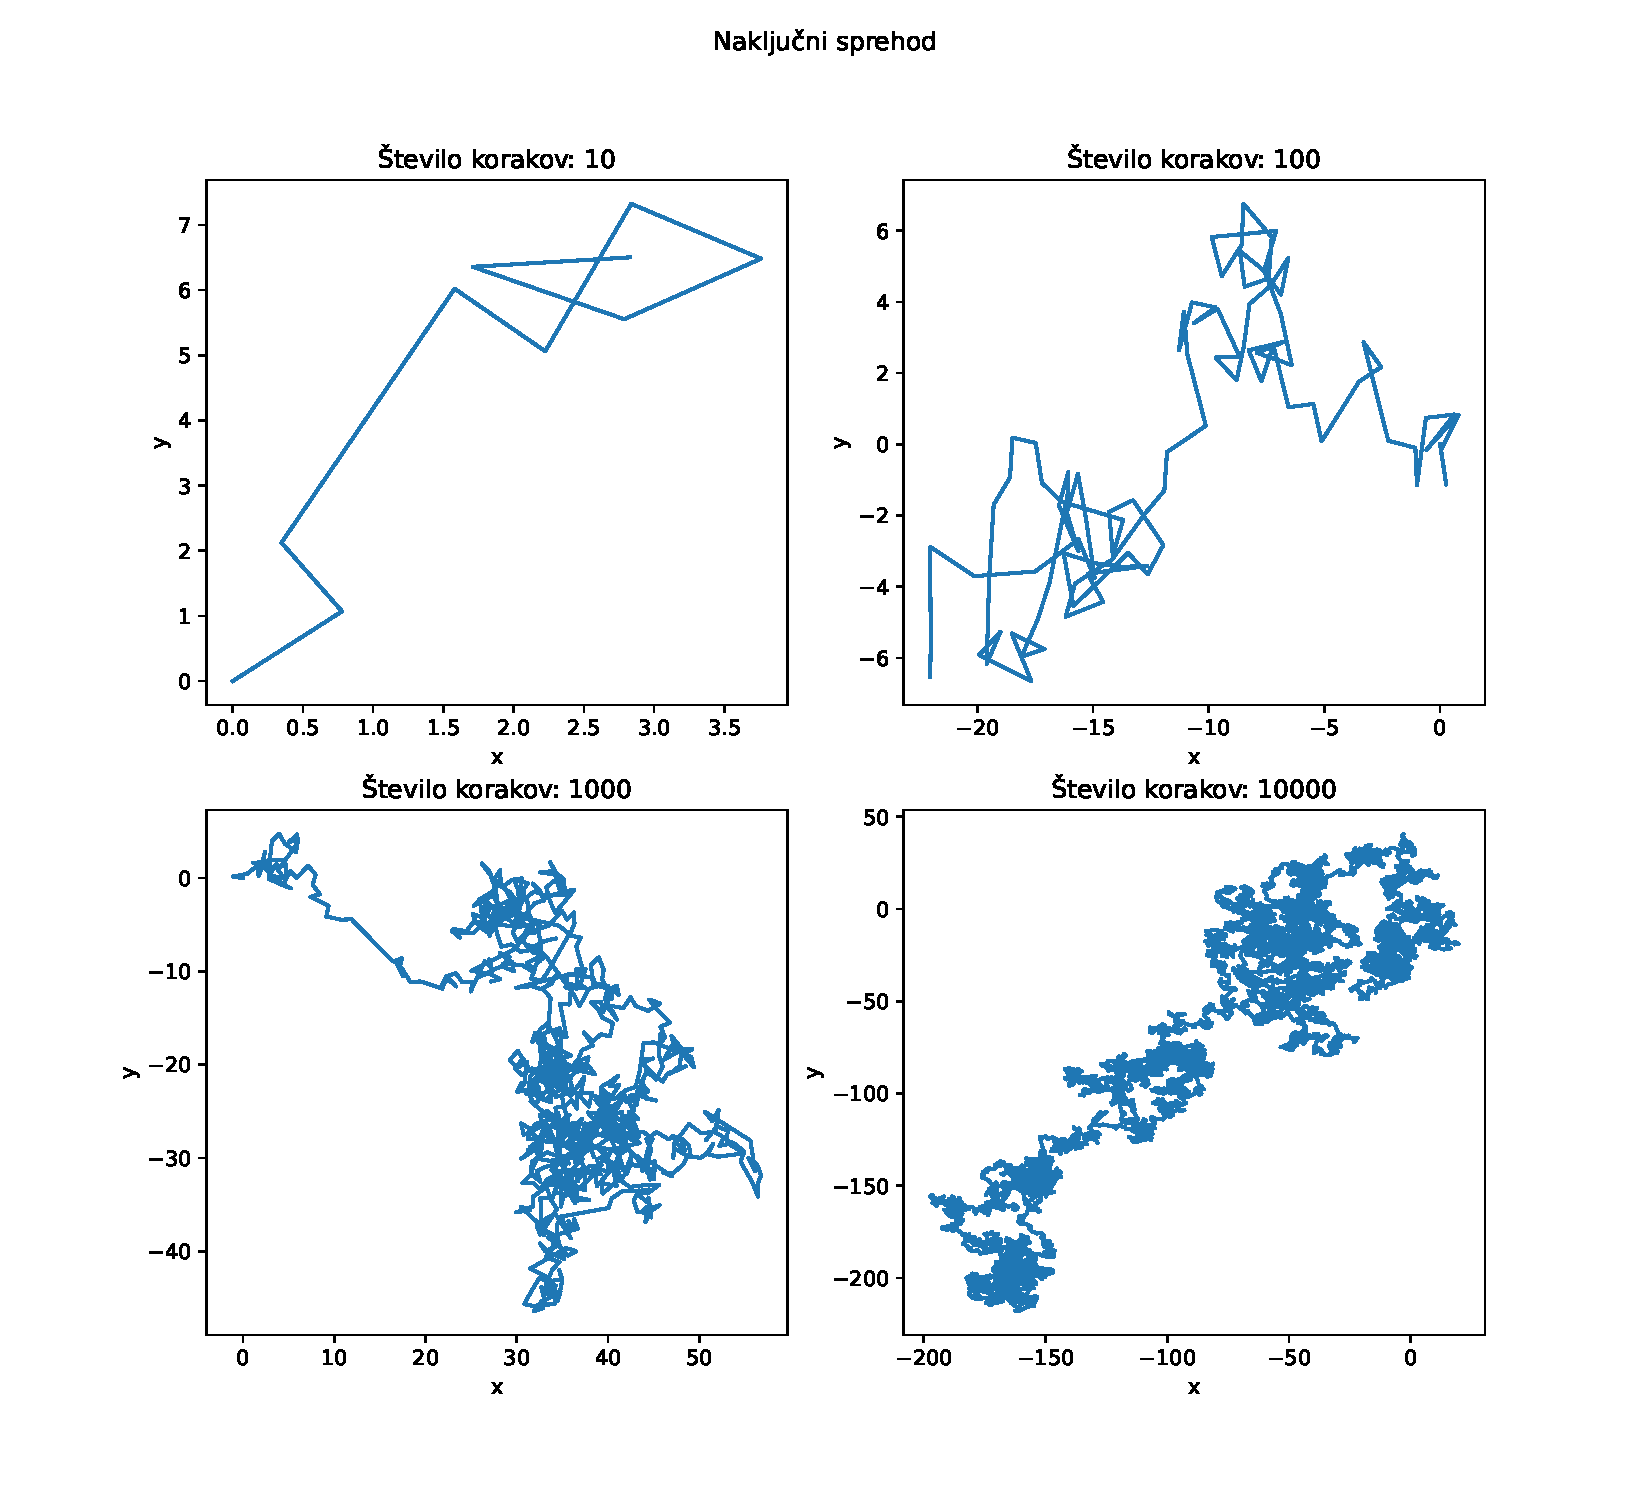
\includegraphics[width=15cm]{nakljucni_sprehodi.pdf}
    \end{center}
    \vspace*{-7mm}
    \caption{Prikaz Levyjevih sprehodov z različnim številom korakov.}
  \end{figure}

Naključne dolžine korakov smo generirali s pomočjo vgrajene funkcije {\sc numpy.random.pareto}, ki vrne 
naključne vrednosti iz potenčne porazdelitve. Namesto vgrajene funkcije pa lahko uporabimo sledečo formulo

\begin{equation*}
  l = (1-\rho)^{-1/(\mu-1)}
\end{equation*}

kjer je $\rho$ naključna spremenljivka porazdeljena enakomerno na intervalu $[0, 1]$. Primerjavo obeh metod prikazuje Graf 2. Zaključimo lahko, da sta obe implementaciji enakovredni.

\begin{figure}[hbtp]
  \begin{center}
  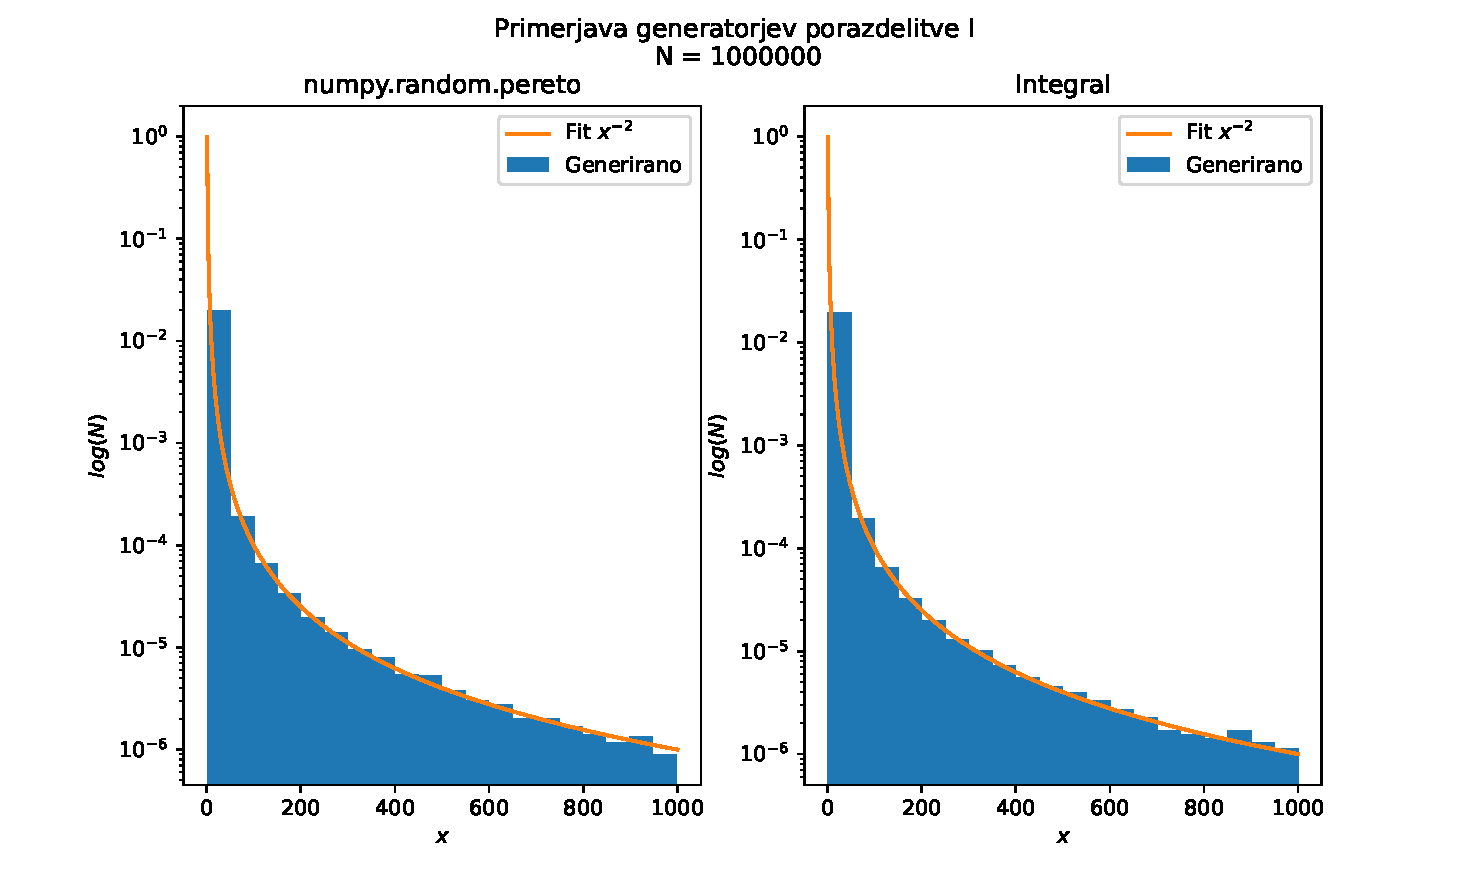
\includegraphics[width=15cm]{prim_gen.pdf}
  \end{center}
  \vspace*{-7mm}
  \caption{Primerjava različnih implementacij generatorjev potenčne porazdelitve.}
\end{figure}

Glavni del naloge je proučiti odvisnost med razpršenostjo sprehodov v odvisnosti od časa. Pri Levyjevih sprehodih časovno odvisnost dobimo direktno s štetjem korakov medtem ko moramo pri poletih izvesti linearno interpolacijo med posameznimi koraki. Interpolacijo izvedemo tako, da najprej izračunamo razliko v času med dvema točkama, s čimer dobimo število točk katere moramo dodati. Nato pa generiramo linearno funkcijo med sosednjima korakoma in odčitamo vmesne vrednosti.

Pri analizi odvisnosti razpršenosti smo na Graf 3 nanašali logaritme vrednosti, kar nam olajša določitev eksponenta $\gamma$, katerega dobimo iz naklona premice. 
Le-te smo nato primerjali z eksponenti uporabljenimi v simulaciji. Kar lahko opazimo je, da se $\gamma_{sim}$ in $\gamma_{fit}$ ne razlikujeta veliko. 
S tem lahko potrdimo teoretično podlago. Na grafu so navedene tudi vrednosti $\sigma^2$, katere so bile pridobljene iz prilagojene premice. Pas napake okoli meritev pa je širine razpršenosti MAD vrednosti. Manjšo napako bi lahko dosegli s povečanjem števila sprehodov in dolžine korakov.

\begin{figure}[hbtp]
  \centering
  \begin{subfigure}{.7\textwidth}
    \centering
    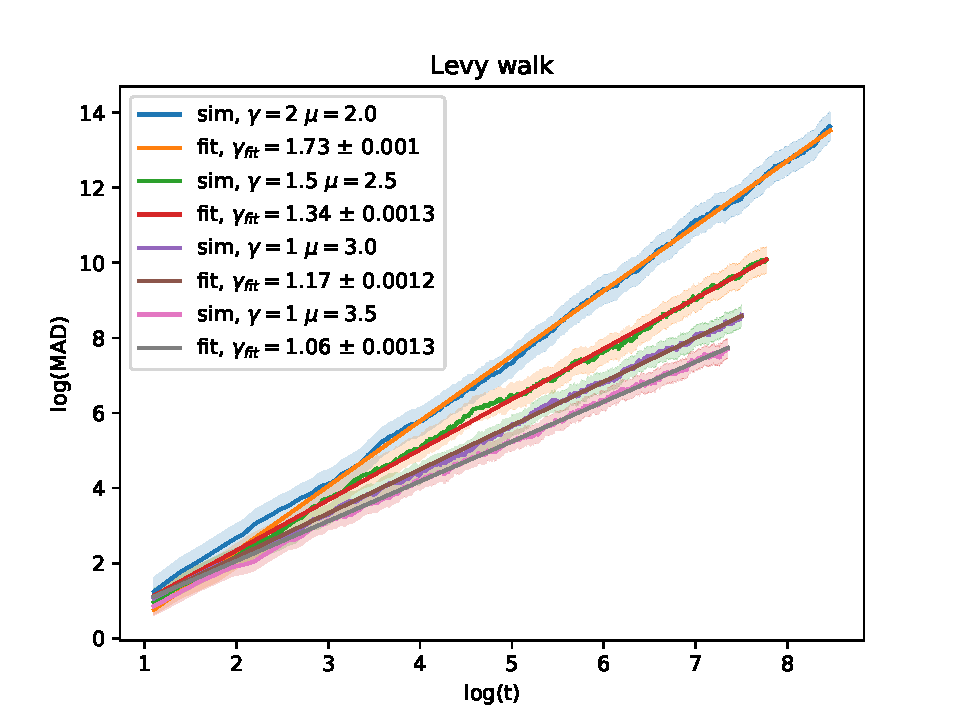
\includegraphics[width=.8\linewidth]{lin_Levy_walk.pdf}
    \caption{Levyjev sprehod}
    \label{fig:sub1}
  \end{subfigure} 
  
  \begin{subfigure}{.7\textwidth}
    \centering
    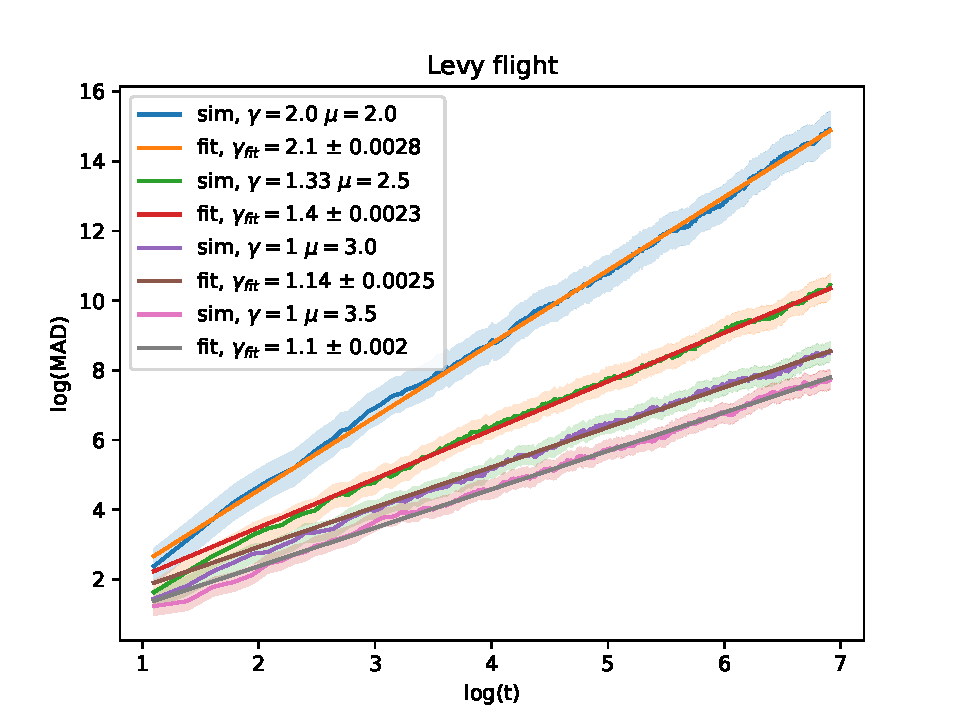
\includegraphics[width=.8\linewidth]{lin_Levy_flight.pdf}
    \caption{Levyjev pobeg}
    \label{fig:sub2}
  \end{subfigure} 
  
  \begin{subfigure}{.7\textwidth}
    \centering
    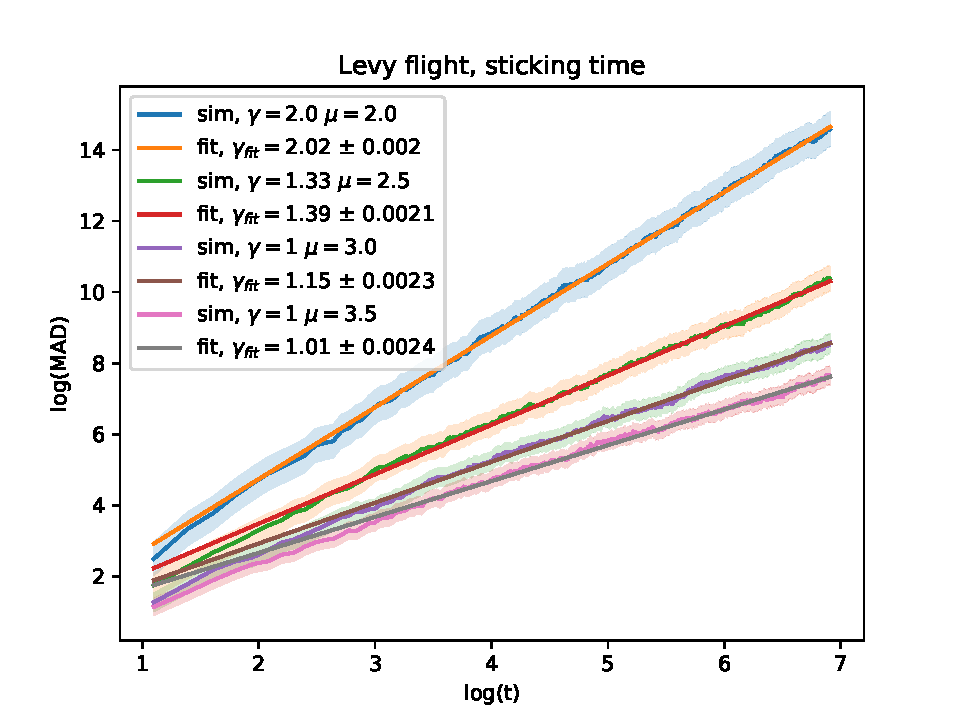
\includegraphics[width=.8\linewidth]{lin_Levy_flight_sticking_time.pdf}
    \caption{Levyjev pobeg s "sticking time"}
    \label{fig:sub3}
  \end{subfigure}
  \caption{Odvisnost MAD od časa pri različnih vrednostih $\mu$. Širina pasu napake je enaka razpršenosti MAD vrednosti.}
  \label{fig:test}
  \end{figure}

  Med seboj pa lahko primerjamo tudi sprehod in pobeg. V grobem je naklon premic nižji pri pobegu. Zaradi načina implementacije pobega nižji naklon sledi iz tega, da za isto število korakov potrebujemo več časa.

  Vsakemu skoku lahko dodamo t.i. "sticing time", ki nam pove koliko časa delec počaka preden naredi naslednji skok. Ta čas je porazdeljen kot; $p(t) \propto t^{-\nu}$, $1 < \nu < 2$. Analizo razpršenosti opravimo tudi na takšnem setu podatkov in opazimo, da ni velike razlike med primerom z in brez uporabe "sticking time".

\section{Zaključek}
Cilj naloge je bilo proučiti obnašanje naključnih sprehodov, bolj specifično Levyjevih sprehodov in poletov. 
Predstavljena rešitev je hiter algoritem za izračun sprehodov in razpršenosti. 
Proučili smo časovno odvisnost razpršenosti ter pokazali ujemanje s teorijo. 
Testirali smo tudi generatorje naključnih števil in generiranje števil iz specifičnih distribucij.

\end{document}

